% !TEX root = ../thesis.tex

\chapter{Erstellung eines featurebasierten Datensets}

\paragraph{Ausblick:}
Dieses Kapitel widmet sich der schrittweisen Erläuterung des Prozesses zur Erstellung des featurebasierten Datensets, welches zur Anlernung der Machine-Learning-Klassifikatoren dient. Dazu wird zunächst die Datenauswahl näher beleuchtet. Darauf folgt eine Darlegung der Konstruktion des Datensets sowie der Auswahl und Berechnung der Metriken, welche als Attribute (Features) im Rahmen der Anlernung der Klassifikatoren dienen. Eine Gliederung der Kapitel kann Abbildung XX entnommen werden.

\begin{figure}[H]
    \centering
    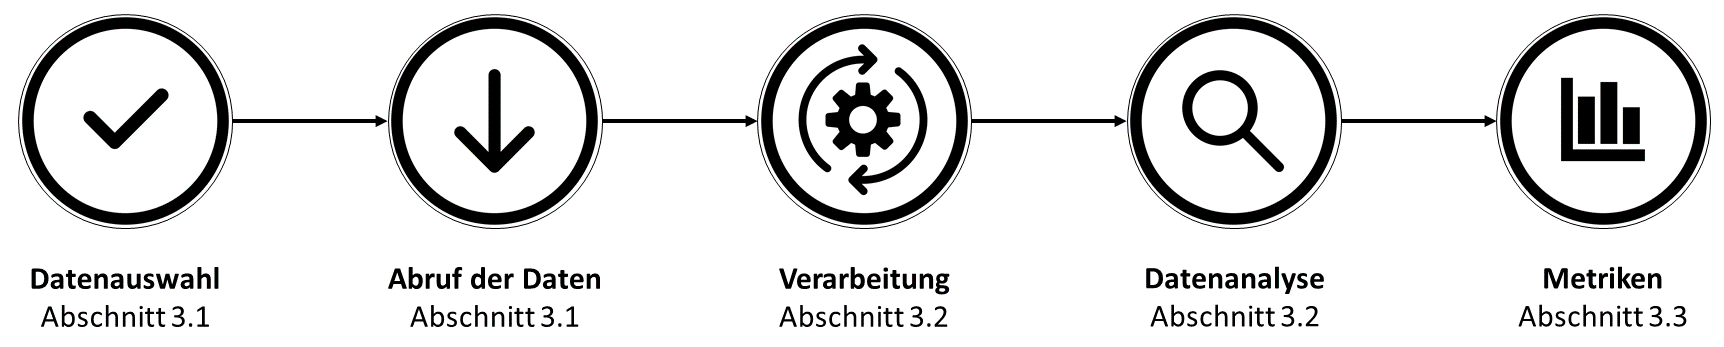
\includegraphics[width=\textwidth]{images/Kap3}
    \caption{Übersicht zur Gliederung des dritten Kapitels\label{fig:kap3}}
\end{figure}

\hrule

\section{Datenauswahl}

Wie im vorangegangenen Kapitel bereits erwähnt wurde, bildet das Datenset die Grundlage für die Anlernung der Machine-Learning-Klassifikatoren und wird eigens für diese Arbeit auf Basis von Commits von 13 featurebasierten Software-Projekten erstellt. Die Auswahl der Software-Projekte erfolge anhand von vorheriger Verwendung in wissenschaftlicher Literatur \cite{Hunsen2015,Liebig2010,Queiroz2016}. Die für diese Arbeit verwendeten Software-Projekte sind samt ihres Einsatzzweckes und ihrer Datenquellen in Tabelle XX aufgeführt.

\begin{table}
\centering
\caption{Übersicht der verwendeten Software-Projekten\protect\footnotemark{}}
\label{tab:tools}
\resizebox{\linewidth}{!}{%
\begin{tabular}{|l|c|c|l|c|c|} 
\cline{2-3}\cline{5-6}
\multicolumn{1}{l|}{} & \textbf{Zweck}       & \textbf{Datenquelle}  &                      & \textbf{Zweck}       & \textbf{Datenquelle}     \\ 
\hline
\textbf{Blender}      & 3D-Modellierungstool & GitHub-Mirror         & \textbf{libxml2}     & XML-Parser           & GitLab-Repository        \\ 
\hline
\textbf{Busybox}      & UNIX-Toolkit         & Git-Repository        & \textbf{lighttpd}    & Webserver            & Git-Repository           \\ 
\hline
\textbf{Emacs}        & Texteditor           & GitHub-Mirror         & \textbf{MPSolve}     & Polynomlöser         & GitHub-Repository        \\ 
\hline
\textbf{GIMP}         & Bildbearbeitung      & GitLab-Repository     & \textbf{Parrot}      & virtuelle Maschine   & GitHub-Repository        \\ 
\hline
\textbf{Gnumeric}     & Tabellenkalkulation  & GitLab-Repository     & \textbf{Vim}         & Texteditor           & GitHub-Repository        \\ 
\hline
\textbf{gnuplot}      & Plotting-Tool        & GitHub-Mirror         & \textbf{xfig}        & Grafikeditor         & Sourceforge-Repository~  \\ 
\hline
\textbf{Irssi}        & IRC-Client           & GitHub-Repository     & \multicolumn{1}{l}{} & \multicolumn{1}{l}{} & \multicolumn{1}{l}{}     \\
\cline{1-3}
\end{tabular}
}
\end{table}
\footnotetext{Links zu den Websites der Softwareprojekte und deren Repositories können im \hyperref[appendix1]{Anhang} eingesehen werden.}

Zum Erhalt der Commit-Daten der Software-Projekte wurde die Python-Library PyDriller\footnote{\href{https://github.com/ishepard/pydriller}{https://github.com/ishepard/pydriller}} verwendet \cite{Spadini2018}. Diese ermöglicht eine einfache Datenextraktion von Git-Repositories zum Erhalt von Commits, Commit-Nachrichten, Entwicklern, Diffs und mehr. Ein beispielhafter Sourcecode-Ausschnitt zur Konsolenausgabe von Metadaten eines Commits (Autor, Name der veränderten Dateien, Typ der Veränderung und jeweilige zyklomatische Komplexität der Dateien) ist in Listing 3.1 aufgeführt. 

\begin{lstlisting}[language=Python, caption=Beispielhafter PyDriller-Code zur Ausgabe von Metadaten von Commits, frame=single]
for commit in RepositoryMining("link_to_repo").traverse_commits(): 
	for m in commit.modifications: 
		print( 
		     "Author {}".format(commit.author.name), 
		     " modified {}".format(m.filename), 
		     " with a change type of {}".format(m.change_type.name), 
		     " and the complexity is {}".format(m.complexity) 
		)
\end{lstlisting}

Als Input der Python-Scripte zum Erhalt der Commit-Daten dienten jeweils die URLs zu den Git-Repositories der Software-Projekte. Weiterhin wurden die Daten in Commits je Release aufgeteilt. Durchgeführt wurde dies durch die Angabe von Release-Tags, basierend auf der Tag-Struktur von Git-Repositories, im PyDriller-Code. Für jede veränderte Datei innerhalb eines Commits und eines Releases wurden die folgenden Metadaten mit Hilfe von PyDriller abgerufen:

\begin{multicols}{2}
\begin{itemize}
\item Commit-Hash (eindeutiger Bezeichner des zugehörigen Commits)
\item Autor des zugehörigen Commits
\item zugehörige Commit-Nachricht
\item Name der veränderten Datei
\item Lines-of-Code der veränderten Datei
\item zyklomatische Komplexität der veränderten Datei
\item Anzahl der hinzugefügten Zeilen zur Datei
\item Anzahl der entfernten Zeilen von der Datei
\item Art der Änderung (ADD, REM, MOD)\footnote{Diese Information fand in der weiteren Erstellung des Datensets keine Verwendung.}
\item Diff der Veränderung
\end{itemize}
\end{multicols}

Die auf diese Weise erhaltenen Daten wurden nach dem Abruf in einer MySQL-Datenbank gespeichert. Für jedes Software-Projekt wurde eine eigene Tabelle erstellt, in welcher neben der oben stehenden Metadaten zudem der Name des betreffenden Software-Projekts und die den Commits zugehörigen Release-Nummern gespeichert wurden. Jede veränderte Datei eines Commits erhält eine Zeile der Datenbank-Tabellen. In Tabelle XX kann eingesehen werden wie viele Releases je Software-Projekt zum Abruf einbezogen wurden und wie viele Commits daraus resultieren.

\begin{table}
\centering
\caption{Übersicht der Anzahl der Releases und Commits je Software-Projekt}
\label{tab:tools}
\resizebox{\linewidth}{!}{%
\begin{tabular}{|l|c|c|l|c|c|} 
\cline{2-3}\cline{5-6}
\multicolumn{1}{l|}{} & \textbf{\#Releases}  & \textbf{\#Commits}  &                      & \multicolumn{1}{l|}{\textbf{\#Releases}~} & \textbf{\#Commits}~   \\ 
\hline
\textbf{Blender}      & 11                   & 19119               & \textbf{libxml2}     & 10                                        & 732                   \\ 
\hline
\textbf{Busybox}      & 14                   & 4984                & \textbf{lighttpd}    & 6                                         & 2597                  \\ 
\hline
\textbf{Emacs}        & 7                    & 12805               & \textbf{MPSolve}     & 8                                         & 668                   \\ 
\hline
\textbf{GIMP}         & 14                   & 7240                & \textbf{Parrot}      & 7                                         & 16245                 \\ 
\hline
\textbf{Gnumeric}     & 8                    & 6025                & \textbf{Vim}         & 7                                         & 9849                  \\ 
\hline
\textbf{gnuplot}      & 5                    & 6619                & \textbf{xfig}        & 7                                         & 18                    \\ 
\hline
\textbf{Irssi}        & 7                    & 253                 & \multicolumn{1}{l}{} & \multicolumn{1}{l}{}                      & \multicolumn{1}{l}{}  \\
\cline{1-3}
\end{tabular}
}
\end{table}

Diese \glqq Rohdaten\grqq{} dienen zur weiteren Verarbeitung hinsichtlich der Erstellung des Datensets und der anschließenden Berechnung der Metriken. Eine Erläuterung der weiteren Verarbeitung der Daten folgt im kommenden Abschnitt.

\begin{table}[]
\caption[Caption for LOF]{Übersicht der zur Erstellung des Datensets verwendeten Software-Projekten mit zugehörigen Werten}
\label{tab:tools}
\resizebox{\textwidth}{!}{%
\begin{tabular}{lccccccc}
                                       & \textbf{Zweck}       & \textbf{Datenquelle}   & \textbf{\#Releases} & \textbf{\#Commits} & \textbf{\#Korrektiv} & \textbf{\#Fehlereinführend} & \textbf{\#Features} \\ \hline
\multicolumn{1}{l|}{\textbf{Blender}}  & 3D-Modellierungstool & GitHub-Mirror          & 11                  & 19119              & 8333                 & 1418                        & 1400         \\
\multicolumn{1}{l|}{\textbf{Busybox}}  & UNIX-Toolkit         & Git-Repository         & 14                  & 4984               & 1408                 & 142                         & 628                 \\
\multicolumn{1}{l|}{\textbf{Emacs}}    & Texteditor           & GitHub-Mirror          & 7                   & 12805              & 6959                 & 685                         & 718                 \\
\multicolumn{1}{l|}{\textbf{GIMP}}     & Bildbearbeitung      & GitLab-Repository      & 14                  & 7240               & 1703                 & 272                         & 204                \\
\multicolumn{1}{l|}{\textbf{Gnumeric}} & Tabellenkalkulation  & GitLab-Repository      & 8                   & 6025               & 1591                 & 136                         & 637                 \\
\multicolumn{1}{l|}{\textbf{gnuplot}}  & Plotting-Tool        & GitHub-Mirror          & 5                   & 6619               & 880                  & 1323                        & 558                 \\
\multicolumn{1}{l|}{\textbf{Irssi}}    & IRC-Client           & GitHub-Repository      & 7                   & 253                & 77                   & 1                           & 9                  \\
\multicolumn{1}{l|}{\textbf{libxml2}}  & XML-Parser           & GitLab-Repository      & 10                  & 732                & 409                  & 37                          & 200                 \\
\multicolumn{1}{l|}{\textbf{lighttpd}} & Webserver            & Git-Repository         & 6                   & 2597               & 1202                 & 555                         & 230                 \\
\multicolumn{1}{l|}{\textbf{MPSolve}}  & Polynomlöser         & GitHub-Repository      & 8                   & 668                & 158                  & 69                          & 54                 \\
\multicolumn{1}{l|}{\textbf{Parrot}}   & Virtuelle Maschine   & GitHub-Repository      & 7                   & 16245              & 3437                 & 824                         & 397                 \\
\multicolumn{1}{l|}{\textbf{Vim}}      & Texteditor           & GitHub-Repository      & 7                   & 9849               & 1033                 & 2571                        & 1158                \\
\multicolumn{1}{l|}{\textbf{xfig}}     & Grafikeditor         & Sourceforge-Repository & 7                   & 18                 & 0                    & 0                           & 137                
\end{tabular}%
}
\end{table}

\fbox{\parbox{\linewidth}{\textit{RQ1a: WELCHE DATEN KOMMEN FÜR DIE ERSTELLUNG DES DATENSETS IN FRAGE?\medskip}\\
Es kommen die Daten von 13 featurebasierten Softwareprojekten zur Verwendung. Mithilfe der Python-Library PyDriller wurden die Metadaten der Commits, aufgeteilt nach Releases, aus den Git-Repositories extrahiert und in MySQL-Datenbanken gespeichert. Ausgewählt wurden die Softwareprojekte aufgrund einer vorherigen Verwendung in der wissenschaftlichen Literatur \cite{Hunsen2015,Liebig2010,Queiroz2016}.}}

\section{Konstruktion des Datensets}

Die Konstruktion des Datensets gliedert sich in mehrere Phasen der Datenverarbeitung und -optimierung. Die erste Phase besteht aus der Extraktion der involvierten Features einer veränderten Datei. Dazu wurden mithilfe eines Python-Scripts die sogenannten Präprozessor-Direktiven \texttt{\#IFDEF} und \texttt{\#IFNDEF} in den Diffs der veränderten Dateien identifiziert und anschließend die den Direktiven folgende Zeichenfolge bis zum Ende der Codezeile als Feature gespeichert. Die Identifizierung erfolgte mittels regulären Ausdrücken. Gespeichert werden die pro Datei identifizierten Features in einer zusätzlichen Spalte in den jeweiligen MySQL-Tabellen der Software-Projekte. Konnte kein Feature identifiziert werden, wird entsprechend \texttt{none} gepseichert.

Dieser Weg der Identifizierung birgt einige Hindernisse. Diese können, neben dem Normalfall, in Abbildung XX gesehen werden. In einigen C-Programmierparadigmen ist es üblich, Header-Dateien mittels Präprozessor-Direktiven in Sourcecode einzubinden, sodass sie wie Features scheinen (siehe erster unerwünschter Fall in Abbildung XX). Diese "Header-Features", wie sie im weiteren Verlauf genannt werden, sollten jedoch ignoriert werden, da sie im Sourcecode keine Variabilität erzeugen. In der Regel sind diese Header-Features identifizierbar durch ihre Namensgebung in Form eines angehängten \texttt{\_h\_} an den Featurenamen, wie beispielsweise \texttt{featurename\_h\_}. Dieser angehängte Teil erlaubt es, die Header-Features mittels regulärer Ausdrücke zu erkennen und auszufiltern. 

Ebenfalls besteht die Möglichkeit, dass \glqq falsche\grqq{} Features identifiziert werden können. Beispiele dafür können von \texttt{\#IFDEFs} stammen, welche in Kommentaren verwendet wurden (siehe zweiter unerwünschter Fall in Abbildung XX). Solche falschen Features wurden in einer manuellen Sichtung der identifizierten Features entfernt und durch \texttt{none} ersetzt.

\begin{figure}[]
    \centering
    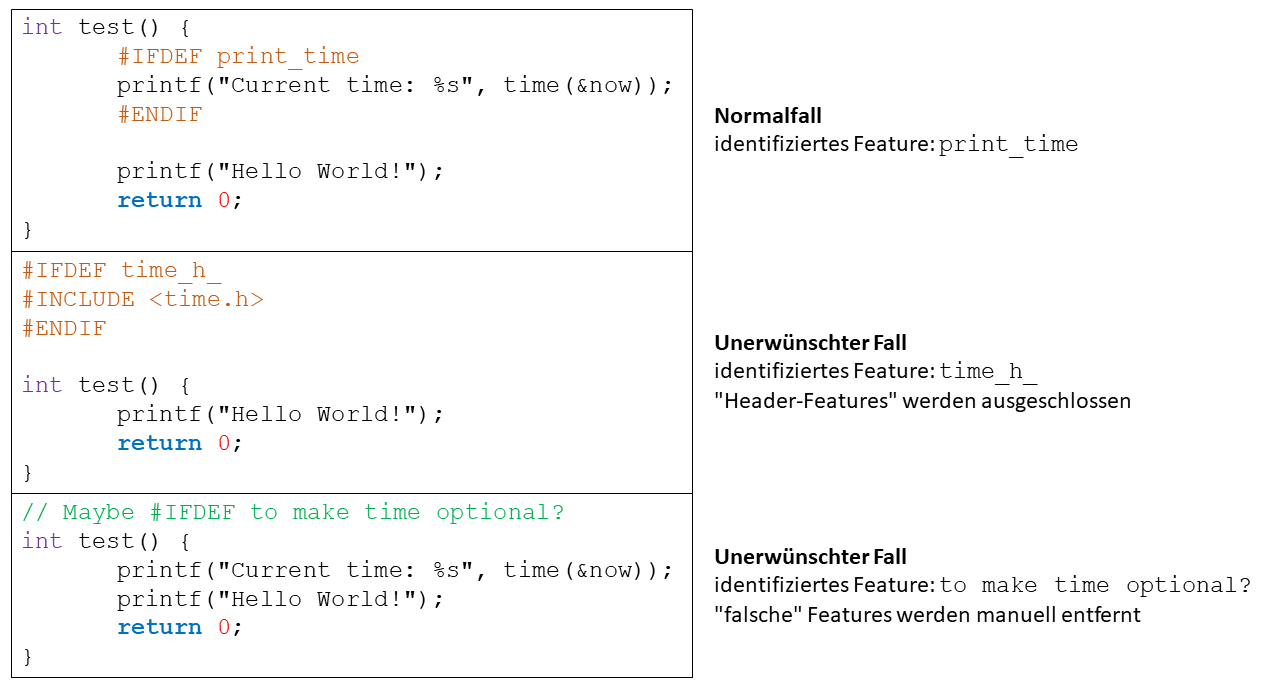
\includegraphics[width=\textwidth]{images/Features}
    \caption{Normalfall und unerwünschte Fälle bei der Identifizierung von Features\label{fig:feat}}
\end{figure}

Die nächste Phase der Verarbeitung besteht aus der Identifizierung von korrektiven Commits. Eine dafür gängige Methode, die auch in dieser Arbeit Anwendung fand, besteht aus der Analyse der Commit-Nachrichten auf das Vorhandensein von bestimmten Schlagworten \cite{Zimmermann2007}. Bei den Schlagworten handelt es sich um \glqq bug\grqq, \glqq error\grqq, \glqq fail\grqq{} und \glqq fix\grqq. Durchgeführt wurde die Analyse mittels Python-Skripte unter Zuhilfenahme von einfachen Formen des Natural Language Processings. Die Ergebnisse wurden in einer weiteren boole'schen Spalte der MySQL-Tabellen (true = korrektiv, false = nicht korrektiv) gespeichert.

\label{szz-def}
Der Suche nach korrektiven Commits folgt eine Analyse nach fehlereinführenden Commits. Dazu wurde eine PyDriller-Implementierung des SZZ-Algorithmus nach Sliwerski, Zimmermann und Zeller verwendet \cite{Sliwerski2005}. Dieser ursprünglich für CVS-Versionskontrollsysteme entwickelte Algorithmus erlaubt es, in zwei Phasen fehlereinführende Commits in lokal gespeicherten Software-Repositories zu finden \cite{Borg2019}. Die erste Phase besteht dabei aus der Identifizierung der korrektiven Commits. Dies kann entweder anhand der zuvor beschriebenen Analyse der Commit-Nachrichten geschehen oder durch die Analyse von Bug-Tracking-Systemen \cite{Borg2019}. Die zweite Phase umfasst die Identifikation der fehlereinführenden Commits auf Basis der zuvor erkannten korrektiven Commits. Diese Phase ist in mehrere Schritte unterteilt und wird in Abbildung XX dargestellt. Die Erläuterungen der mit Buchstaben versehenen Schritte erfolgt im Anschluss. Die PyDriller-Implementierung des Algorithmus folgt dem gezeigten Ablauf.

\begin{figure}[]
    \centering
    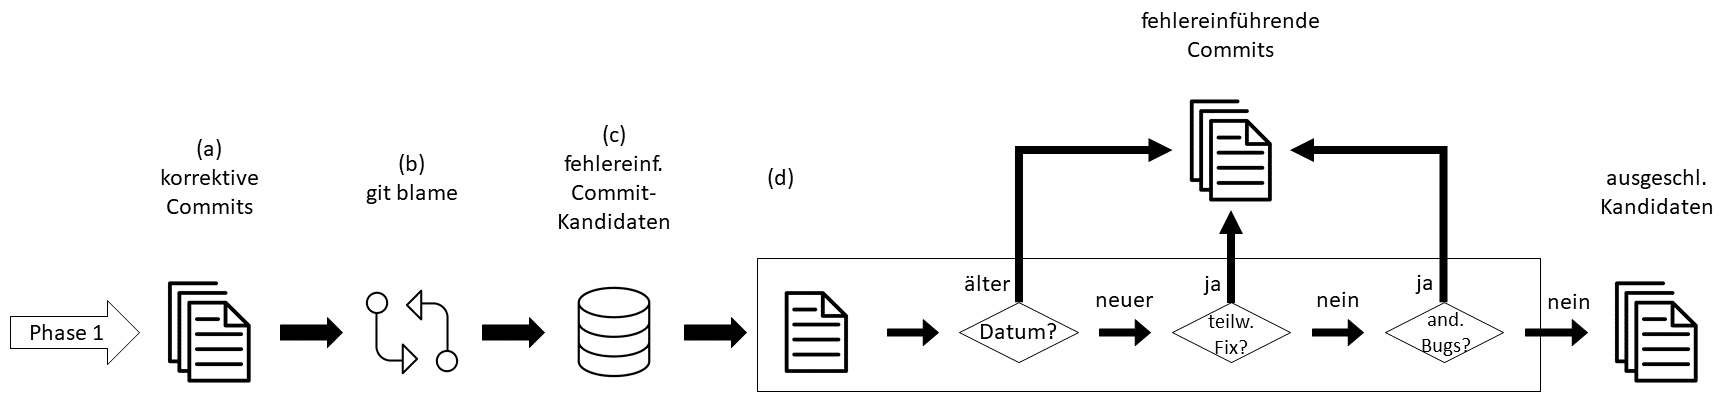
\includegraphics[width=\textwidth]{images/SZZ}
    \caption{Ablauf der zweiten Phase des SZZ-Algorithmus (übersetzt, \cite{Borg2019})\label{fig:szz}}
\end{figure}

Die zweite Phase des SZZ-Algorithmus, die als Input eine Liste der Commit-Hashes der zuvor erkannten korrektiven Commits (a) erhält, beginnt mit der Ausführung eines \texttt{git blame} Befehls (b) zur Identifizierung sämtlicher Commits, in denen Veränderungen an den selben Dateien und Codezeilen vorgenommen wurden wie in den korrektiven Commits \cite{Borg2019}. Daraus resultieren mögliche fehlereinführende Commit-Kandidaten (c). Für jeden dieser Commit-Kandidaten wird dann erörtert, ob er fehlereinführend ist (d). Dazu wird zunächst das Datum des Commit-Kandidaten mit dem zugehörigen korrektiven Commits verglichen. Liegt dieses vor dem Datum des korrektiven Commits, so gilt der Kandidat als tatsächlich fehlereinführend \cite{Borg2019}. Liegt das Datum danach, so kann der Kandidat nur fehlereinführend sein, sofern er teilweise den vorhandenen Fehler löst (teilweiser Fix) oder für einen anderen Fehler verantwortlich ist, der nicht dem korrektiven Commit zugehörig ist (Kandidat ist Fehlerursache eines anderen korrektiven Commits) \cite{Borg2019}. Die Ausgabe ist eine Liste von Commit-Hashes von fehlereinführenden Commits für jeden korrektiven Commit. Diese neuen Informationen werden in einer zusätzlichen boole'schen Spalte in den MySQL-Tabellen gespeichert (true = fehlereinführend, false = nicht fehlereinführend). 

Eine Übersicht des Schemas der nun vollständigen initialen  MySQL-Tabellen (im folgenden Haupttabellen genannt) ist in Tabelle XX aufgeührt. Wie bereits zuvor erwähnt, umfasst diese Tabellle für jede veränderte Datei eines Commits eine Ziele. Sollten in einem Diff einer veränderten Datei mehrere Features identifiziert worden sein, so wird für jedes Feature die entsprechende Zeile dupliziert.

\begin{table}
\centering
\caption{Übersicht des Schemas der MySQL-Haupttabellen}
\label{tab:schema1}
\resizebox{\linewidth}{!}{%
\begin{tabular}{|ll|ll|} 
\hline
\textbf{Spaltenname}  & \textbf{Beschreibung}                                                                               & \textbf{Spaltenname}  & \textbf{Beschreibung}                                                                             \\ 
\hline
name                  & Name des Softwareprojekts                                                                           & lines\_added          & \begin{tabular}[c]{@{}l@{}}Anzahl der hinzugefügten Zeilen\\ zur geänderten Datei \end{tabular}   \\
release\_number       & \begin{tabular}[c]{@{}l@{}}zugehörige Release-Version\\ basierend auf vergebenen Tags \end{tabular} & lines\_removed        & \begin{tabular}[c]{@{}l@{}}Anzahl der entfernten Zeilen\\ von der geänderten Datei \end{tabular}  \\
commit\_hash          & \begin{tabular}[c]{@{}l@{}}eindeutiger Bezeichner eines \\ Commits \end{tabular}                    & change\_type          & Art der Änderung                                                                                  \\
commit\_author        & Autor eines Commits                                                                                 & diff                  & Diff der geänderten Datei                                                                         \\
commit\_msg           & Nachricht eines Commits                                                                             & corrective            & \begin{tabular}[c]{@{}l@{}}Indikator, ob Commit\\ fehlerbehebend war \end{tabular}                \\
filename              & Name der geänderten Datei                                                                           & bug\_introducing      & \begin{tabular}[c]{@{}l@{}}Indikator, ob Commit\\ fehlereinführend war \end{tabular}              \\
nloc                  & \begin{tabular}[c]{@{}l@{}} „ Lines of code“ der geänderten\\ Datei \end{tabular}                   & feature               & \begin{tabular}[c]{@{}l@{}}Namen der zugehörigen Features\\ der geänderten Datei \end{tabular}    \\
cycomplexity          & \begin{tabular}[c]{@{}l@{}}Zyklomatische Komplexität\\ der geänderten Datei \end{tabular}           &                       &                                                                                                   \\
\hline
\end{tabular}
}
\end{table}

Auf Basis der Daten der Haupttabellen können nun die für das Training der Klassifikatoren benötigten Metriken berechnet werden.

\section{Metriken}

Wie bereits in Kapitel XX erwähnt wurde, bilden sogenannte Metriken die Attribute zum Training der Machine-Learning-Klassifikatoren. Bei Metriken handelt sich sich um Zahlenwerte, die in Codemetriken und Prozessmetriken aufgeteilt sind und jeweils anhand der vorhandenen Daten des Datensets berechnet werden \cite{Rahman2013}. Codemetriken werden genutzt um Eigenschaften von Sourcecode, wie zum Beispiel \glqq Größe\grqq{} oder Komplexität, zu messen \cite{Rahman2013}. Prozessmetriken dienen hingegen zur Messung von Eigenschaften, die anhand von Metadaten aus Software-Repositories erörtert werden können \cite{Rahman2013}. Beispiele dafür sind Anzahl der Veränderungen einer bestimmten Datei oder Anzahl der aktiven Entwickler an einem Projekt. Für diese Arbeit wurden 11 Metriken errechnet, aufgeteilt in 7 Prozess- und 4 Codemetriken. Fünf der Prozessmetriken wurden aus wissenschaftlichen Arbeiten \cite{Rahman2013,Queiroz2016} entnommen. Die weiteren sechs Metriken wurden auf Basis der von PyDriller erhaltenen Metadaten der Commits berechnet.

Im Hinblick auf die spätere Evaluation der Arbeit wurden die Metriken nicht nur auf Basis von Features sondern auch auf Basis von Dateien berechnet. Der letztgenannte Ansatz stellt die in der Machine-Learning-gestützten Fehlererkennung üblicherweise verwendete Methodik dar. Diese beiden Ansätze können somit im Rahmen der Evaluation verglichen werden. Für die Berechnung der dateibasierten Metriken mussten die Daten der Haupttabellen nicht weiter verarbeitet werden, da die erforderlichen Metadaten der Dateien bereits mit PyDriller abgerufen wurden, da sie die Grundlage der Identifikation der Features bildeten. In Abbildung XX wird die Abgrenzung zwischen feature- und dateibasierten Datensets anhand des Ablaufs der Verarbeitung der Rohdaten von PyDriller visualisiert. Es ist zu erkennen, dass für die Berechnung der dateibasierten Metriken keine weiteren Verarbeitungsschritte (Schritte A + B) nötig sind. Lediglich zur Herstellung des Featurebezugs sind weitere Schritte nötig, welche bereits im vorherigen Abschnitt erläutert wurden (Schritte C - E). Die finalen Datensets (G) bestehen aus den jeweils berechneten feature- und dateibezogenen Metriken (E) sowie den Labeln der Zielklasse. Eine Übersicht der berechneten Metriken samt Beschreibung befindet sich in Tabelle XX.

\begin{figure}[]
    \centering
    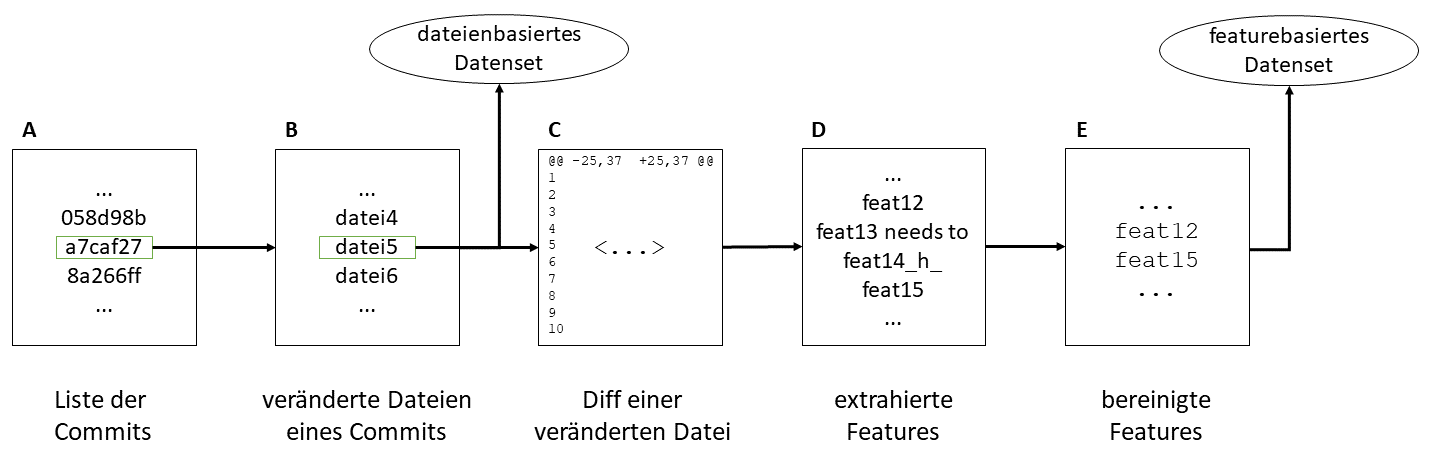
\includegraphics[width=\textwidth]{images/Dataset}
    \caption{Visualisierung des Aufbaus und Unterscheidung der Datensets\label{fig:dataset}}
\end{figure}

\begin{table}
\centering
\caption{Übersicht der berechneten Metriken}
\label{tab:metrics}
\resizebox{\linewidth}{!}{%
\begin{tabular}{l|llc} 
\cline{2-4}
                             & \textbf{Metrik}                                                                               & \textbf{Beschreibung}                                                                                                                                                                                                                                                                                                                                        & \multicolumn{1}{c|}{\textbf{Quelle} }  \\ 
\hline
\multirow{7}{*}{\textbf{\parbox[t]{2mm}{\multirow{3}{*}{\rotatebox[origin=c]{90}{Prozessmetriken}}}}} & Anzahl der~Commits (COMM)                                                                     & Anzahl der Commits, die dem Feature / der Datei in einem Release zugeordnet sind.                                                                                                                                                                                                                                                                            & \cite{Rahman2013,Queiroz2016}                                    \\
                             & \begin{tabular}[c]{@{}l@{}}Anzahl der\\aktiven Entwickler (ADEV)\end{tabular}                 & \begin{tabular}[c]{@{}l@{}}Anzahl der Entwickler, die innerhalb eines Releases das Feature /\\die Datei bearbeitet (geändert, gelöscht oder hinzugefügt) haben.\end{tabular}                                                                                                                                                                                 & \cite{Rahman2013,Queiroz2016}                                    \\
                             & \begin{tabular}[c]{@{}l@{}}eindeutige\\Entwickleranzahl (DDEV)\end{tabular}                   & \begin{tabular}[c]{@{}l@{}}kumulierte Anzahl der Entwickler, die innerhalb eines Releases das Feature / \\die Datei bearbeitet (geändert, gelöscht oder hinzugefügt) haben.\end{tabular}                                                                                                                                                                     & \cite{Rahman2013,Queiroz2016}                                    \\
                             & \begin{tabular}[c]{@{}l@{}}Erfahrung~aller\\Entwickler (EXP)\end{tabular}                     & \begin{tabular}[c]{@{}l@{}}geometrisches Mittel der \glqq Erfahrung\grqq{} aller Entwickler, die innerhalb eines Releases\\das Feature /~die Datei bearbeitet (geändert, gelöscht oder hinzugefügt) haben. \\Erfahrung ist definiert als Summe der geänderten, gelöschten oder hinzugefügten \\Zeilen in den dem Feature / der Datei zugeordneten Commits. \end{tabular} & \cite{Rahman2013,Queiroz2016}                                    \\
                             & \begin{tabular}[c]{@{}l@{}}Erfahrung des meist \\beteiligten Entwicklers\\(OEXP)\end{tabular} & \begin{tabular}[c]{@{}l@{}}\glqq Erfahrung\grqq{} des Entwicklers, die innerhalb eines Releases das Feature / die Datei \\am häufigsten bearbeitet (geändert, gelöscht oder hinzugefügt) hat.\\Erfahrung ist definiert als Summe der geänderten, gelöschten oder hinzugefügten\\Zeilen in den dem Feature / der Datei zugeordneten Commits. \end{tabular}                & \cite{Rahman2013,Queiroz2016}                                    \\
                             & \begin{tabular}[c]{@{}l@{}}Grad der\\Änderungen (MODD)\end{tabular}                           & \begin{tabular}[c]{@{}l@{}}Anzahl der Bearbeitungen (Änderung, Entfernung, Erweiterung) des Features /\\der Datei innerhalb eines Releases.\end{tabular}                                                                                                                                                                                                     & neu                                    \\
                             & \begin{tabular}[c]{@{}l@{}}Umfang der\\Änderungen (MODS)\end{tabular}                         & \begin{tabular}[c]{@{}l@{}}Anzahl der bearbeiteten Features / Dateien innerhalb eines Releases \\(Feature- bzw. dateiübergreifender Wert). Idee: Je mehr Features / \\Dateien in einem Release bearbeitet worden, desto fehleranfälliger scheinen \\diese zu sein. \end{tabular}                                                                             & neu                                    \\ 
\hline
\multirow{4}{*}{\textbf{\parbox[t]{2mm}{\multirow{3}{*}{\rotatebox[origin=c]{90}{Codemetriken}}}}} & \begin{tabular}[c]{@{}l@{}}Anzahl der\\Codezeilen (NLOC)\end{tabular}                         & \begin{tabular}[c]{@{}l@{}}Durchschnittliche Anzahl der Codezeilen der dem Feature \\zugeordneten Dateien / der Datei innerhalb eines Releases.\end{tabular}                                                                                                                                                                                                 & neu                                    \\
                             & \begin{tabular}[c]{@{}l@{}}Zyklomatische\\Komplexität (CYCO)\end{tabular}                     & \begin{tabular}[c]{@{}l@{}}Durchschnittliche zyklomatische Komplexität der dem Feature \\zugeordneten Dateien / der Datei innerhalb eines Releases.\end{tabular}                                                                                                                                                                                             & neu                                    \\
                             & \begin{tabular}[c]{@{}l@{}}Anzahl der\\hinzugefügten Zeilen (ADDL)\end{tabular}               & \begin{tabular}[c]{@{}l@{}}Durchschnittliche Anzahl der hinzugefügten Codezeilen zu den dem Feature\\zugeordneten Dateien / zur Datei innerhalb eines Releases.\end{tabular}                                                                                                                                                                                 & neu                                    \\
                             & \begin{tabular}[c]{@{}l@{}}Anzahl der\\entfernten Zeilen (REML)\end{tabular}                  & \begin{tabular}[c]{@{}l@{}}Durchschnittliche Anzahl der gelöschten Codezeilen von den dem Feature\\zugeordneten Dateien /~ von der Datei innerhalb eines Releases.\end{tabular}                                                                                                                                                                              & neu                                   
\end{tabular}
}
\end{table}

\begin{table}
\centering
\caption{Overview of used metrics}
\label{tab:metrics}
\resizebox{\linewidth}{!}{%
\begin{tabular}{l|llc} 
\cline{2-4}
                             & \textbf{Metric}                                                                            & \textbf{Description}                                                                                                                                                                                                                                                                                        & \multicolumn{1}{c|}{\textbf{Source} }  \\ 
\hline
\multirow{7}{*}{\textbf{\rotatebox[origin=c]{90}{Process metrics}}} & Number of commits (COMM)                                                                   & Number of commits associated with the feature/file in a release.                                                                                                                                                                                                                                             & \cite{Rahman2013,Queiroz2016}                                    \\
                             & Number of active developers (ADEV)                                                         & \begin{tabular}[c]{@{}l@{}}Number of developers who have edited (changed, deleted or added) \\the feature / file within a release\end{tabular}                                                                                                                                                               & \cite{Rahman2013,Queiroz2016}                                    \\
                             & Number of distinct developers (DDEV)                                                       & \begin{tabular}[c]{@{}l@{}}Cumultative number of developers who have edited (changed, deleted or added) \\the feature / file within a release\end{tabular}                                                                                                                                                   & \cite{Rahman2013,Queiroz2016}                                    \\
                             & Experience of all develepoers (EXP)                                                        & \begin{tabular}[c]{@{}l@{}}geometric mean of the experience of all developers who have edited \\(changed, deleted or added) the feature / file within a release.~\\Experience is defined as the sum of the changed, deleted or added \\lines in the commits associated with the feature / file.\end{tabular} & \cite{Rahman2013,Queiroz2016}                                    \\
                             & \begin{tabular}[c]{@{}l@{}}Experience of the most involved developers\\(OEXP)\end{tabular} & \begin{tabular}[c]{@{}l@{}}Experience of the developer who has edited (changed, deleted or added) \\the feature / file most often within a release. Experience is defined as the \\sum of changed, deleted, or added lines in the commits associated with the \\feature/file.\end{tabular}                   & \cite{Rahman2013,Queiroz2016}                                    \\
                             & Degree of modifications (MODD)                                                             & Number of edits (change, removal, extension) of the feature / file within a release.                                                                                                                                                                                                                         & new                                    \\
                             & Scope of modifications (MODS)                                                              & \begin{tabular}[c]{@{}l@{}}Number of edited features / files within a release (feature or file overlapping value). \\Idea: The more features / files have been edited in a release, \\the more error-prone they seem to be.\end{tabular}                                                                     & new                                    \\ 
\hline
\multirow{4}{*}{\textbf{\rotatebox[origin=c]{90}{Code metrics}}} & Lines of code (NLOC)                                                                       & \begin{tabular}[c]{@{}l@{}}Average number of lines of code of the files associated with the feature /\\~file within a release.\end{tabular}                                                                                                                                                                  & new                                    \\
                             & Cyclomatic Complexity (CYCO)                                                               & \begin{tabular}[c]{@{}l@{}}Average cyclomatic complexity of the files associated with the feature / \\file within a release.\end{tabular}                                                                                                                                                                    & new                                    \\
                             & Number of added lines (ADDL)                                                               & \begin{tabular}[c]{@{}l@{}}Average number of lines of code added to the files associated with \\the feature / file within a release.\end{tabular}                                                                                                                                                            & new                                    \\
                             & Number of removed lines (REML)                                                             & \begin{tabular}[c]{@{}l@{}}Average number of lines of code deleted from the files associated \\with the feature / from the file within a release\end{tabular}                                                                                                                                                & new                                   
\end{tabular}
}
\end{table}

\begin{table}[]
\caption{Übersicht des Schemas der Metrics-Tabellen des Datensets}
\label{tab:schema2}
\resizebox{\textwidth}{!}{%
\begin{tabular}{ll|ll}
\textbf{Spaltenname} & \textbf{Beschreibung}                                                                                                                                                                          & \textbf{Spaltenname} & \textbf{Beschreibung}                                                                                                                                                           \\ \hline
name                 & Name des Softwareprojekts                                                                                                                                                                      & oexp                 & \begin{tabular}[c]{@{}l@{}}"Erfahrung" des Entwicklers, der am\\ meisten zum betreffenden Feature / \\ zur betreffenden Datei in  einem Release \\ beigetragen hat\end{tabular} \\
release\_number      & \begin{tabular}[c]{@{}l@{}}zugehörige Release-Version\\ basierend auf vergebene Tags\end{tabular}                                                                                              & scat                 & \begin{tabular}[c]{@{}l@{}}Scattering Degree des betreffenden Features / \\ der betreffenden Datei\end{tabular}                                                                 \\
feature / filename   & \begin{tabular}[c]{@{}l@{}}betreffendes Feature / \\ betreffende Datei\end{tabular}                                                                                                            & tang                 & \begin{tabular}[c]{@{}l@{}}Tangling Degree des betreffenden Features / \\ der betreffenden Datei\end{tabular}                                                                   \\
comm                 & \begin{tabular}[c]{@{}l@{}}Anzahl der Commits, die in einem\\ Release dem betreffenden Feature / \\ der betroffenen Datei gewidmet sind\end{tabular}                                           & nloc                 & \begin{tabular}[c]{@{}l@{}}Durchschnittliche Lines of Code der Bearbeitungen \\ des betreffenden Features / der betreffenden Datei\\ in einem Release\end{tabular}              \\
adev                 & \begin{tabular}[c]{@{}l@{}}Anzahl der Entwickler, die das\\ betreffende Feature / die betreffende \\ Datei in einem Release bearbeitet haben\end{tabular}                                      & cyco                 & \begin{tabular}[c]{@{}l@{}}Durchschnittliche zyklomatische Komplexität der \\ Bearbeitungen  des betreffenden Features /\\ der betreffenden Datei in einem Release\end{tabular} \\
ddev                 & \begin{tabular}[c]{@{}l@{}}kummulierte Anzahl der Entwickler, \\ die das betreffende Feature / \\ die betreffende Datei in einem\\ Release bearbeitet haben\end{tabular}                       & addl                 & \begin{tabular}[c]{@{}l@{}}Durchschnittliche Anzahl der hinzugefügten Zeilen \\ des betreffenden Features / der betreffenden Datei\\ in einem Release\end{tabular}              \\
exp                  & \begin{tabular}[c]{@{}l@{}}Geometrisches Mittel der "Erfahrung"\\ aller Entwickler, die am betreffenden\\ Feature / an der betreffenden Datei\\ in einem Release gearbeitet haben\end{tabular} & reml                 & \begin{tabular}[c]{@{}l@{}}Durchschnittliche Anzahl der entfernten Zeilen \\ des betreffenden Features / der betreffenden Datei\\ in einem Release\end{tabular}                
\end{tabular}%
}
\end{table}

\fbox{\parbox{\linewidth}{\textit{RQ1b: WIE WEIT MÜSSEN DIE DATEN VORVERARBEITET WERDEN, UM SIE FÜR DAS TRAINING NUTZBAR ZU MACHEN?\medskip}\\
Eine umfassende Vorverarbeitung der Daten aus den Repositories ist nicht nötig. Die Verarbeitungsschritte bestanden aus: Extraktion der Features inklusive Bereinigung, Identifizierung von korrektiven Commits mittels Analyse der Commit-Nachrichten, Analyse nach fehlereinführenden Commits unter Zuhilfenahme des SZZ-Algorithmus sowie Berechnung von elf Metriken, welche als Attribute für die Erlernung der Klassifikatoren dienen.}}

\cleardoublepage